\documentclass[tikz,convert={density=150,size=600,outext=.png}]{standalone}
\usetikzlibrary{shapes, calc, arrows, fit, positioning, decorations, patterns, decorations.pathreplacing, chains, snakes}
\input{../setup-web-fonts}
\input{../setup-packages}
\graphicspath{{../pictures/}} % path to pictures, trailing slash is mandatory.

% The actual drawing follows
\begin{document}
    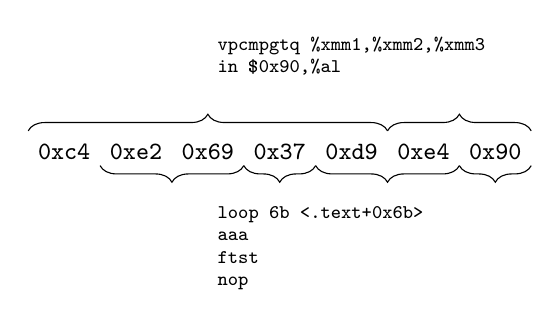
\begin{tikzpicture}[>=latex]

    \begin{scope}[start chain, node distance = 0cm, font=\ttfamily\small, every node/.style={on chain}]
        \node[align=left] (byte0) {0xc4};
        \node[align=left] (byte1) {0xe2};
        \node[align=left] (byte2) {0x69};
        \node[align=left] (byte3) {0x37};
        \node[align=left] (byte4) {0xd9};
        \node[align=left] (byte5) {0xe4};
        \node[align=left] (byte6) {0x90};
    \end{scope}
    
    \node[below= of byte2, anchor = west, align=left, font=\ttfamily\scriptsize]  (var1) {loop   6b <.text+0x6b> \\ aaa \\ ftst \\ nop};
    
    \node[above= of byte2, anchor = west, align=left, font=\ttfamily\scriptsize]  (var2) { vpcmpgtq \%xmm1,\%xmm2,\%xmm3 \\ in     \$0x90,\%al};
    
    \draw[decorate, decoration={brace, amplitude=6pt}] ([yshift=0.05cm] byte0.north west) -- ([yshift=0.05cm] byte4.north east);
    \draw[decorate, decoration={brace, amplitude=6pt}] ([yshift=0.05cm] byte5.north west) -- ([yshift=0.05cm] byte6.north east);
    
    \draw[decorate, decoration={brace, amplitude=6pt}] ([yshift=0.05cm] byte2.south east) -- ([yshift=0.05cm] byte1.south west);
    \draw[decorate, decoration={brace, amplitude=6pt}] ([yshift=0.05cm] byte3.south east) -- ([yshift=0.05cm] byte3.south west);
    \draw[decorate, decoration={brace, amplitude=6pt}] ([yshift=0.05cm] byte5.south east) -- ([yshift=0.05cm] byte4.south west);
    \draw[decorate, decoration={brace, amplitude=6pt}] ([yshift=0.05cm] byte6.south east) -- ([yshift=0.05cm] byte6.south west);
    
    \end{tikzpicture}

\end{document}
